\section{Ships, Spacelanes, and Path Finding}
\label{sec:pathfinding}

The specification made it clear --- by the way weapons and navigation between planets was to be structured --- that ship motion needed to be relatively detailed. It is no use having a weapon that can be only used in one arc if ships could instantly pivot on the spot. Instead it was desired for ships to move as large objects with a great deal of momentum, with large turning circles and ponderous movements. However it would be undesirable for the motion of ships to be too realistic, as it would make the game needlessly difficult and confusing. A real object undergoing acceleration in space could of course, accelerate essentially indefinitely (until it was nearing the speed of light) but would need to take an equal amount of time to decelerate to stop again.

\begin{marginfigure}
	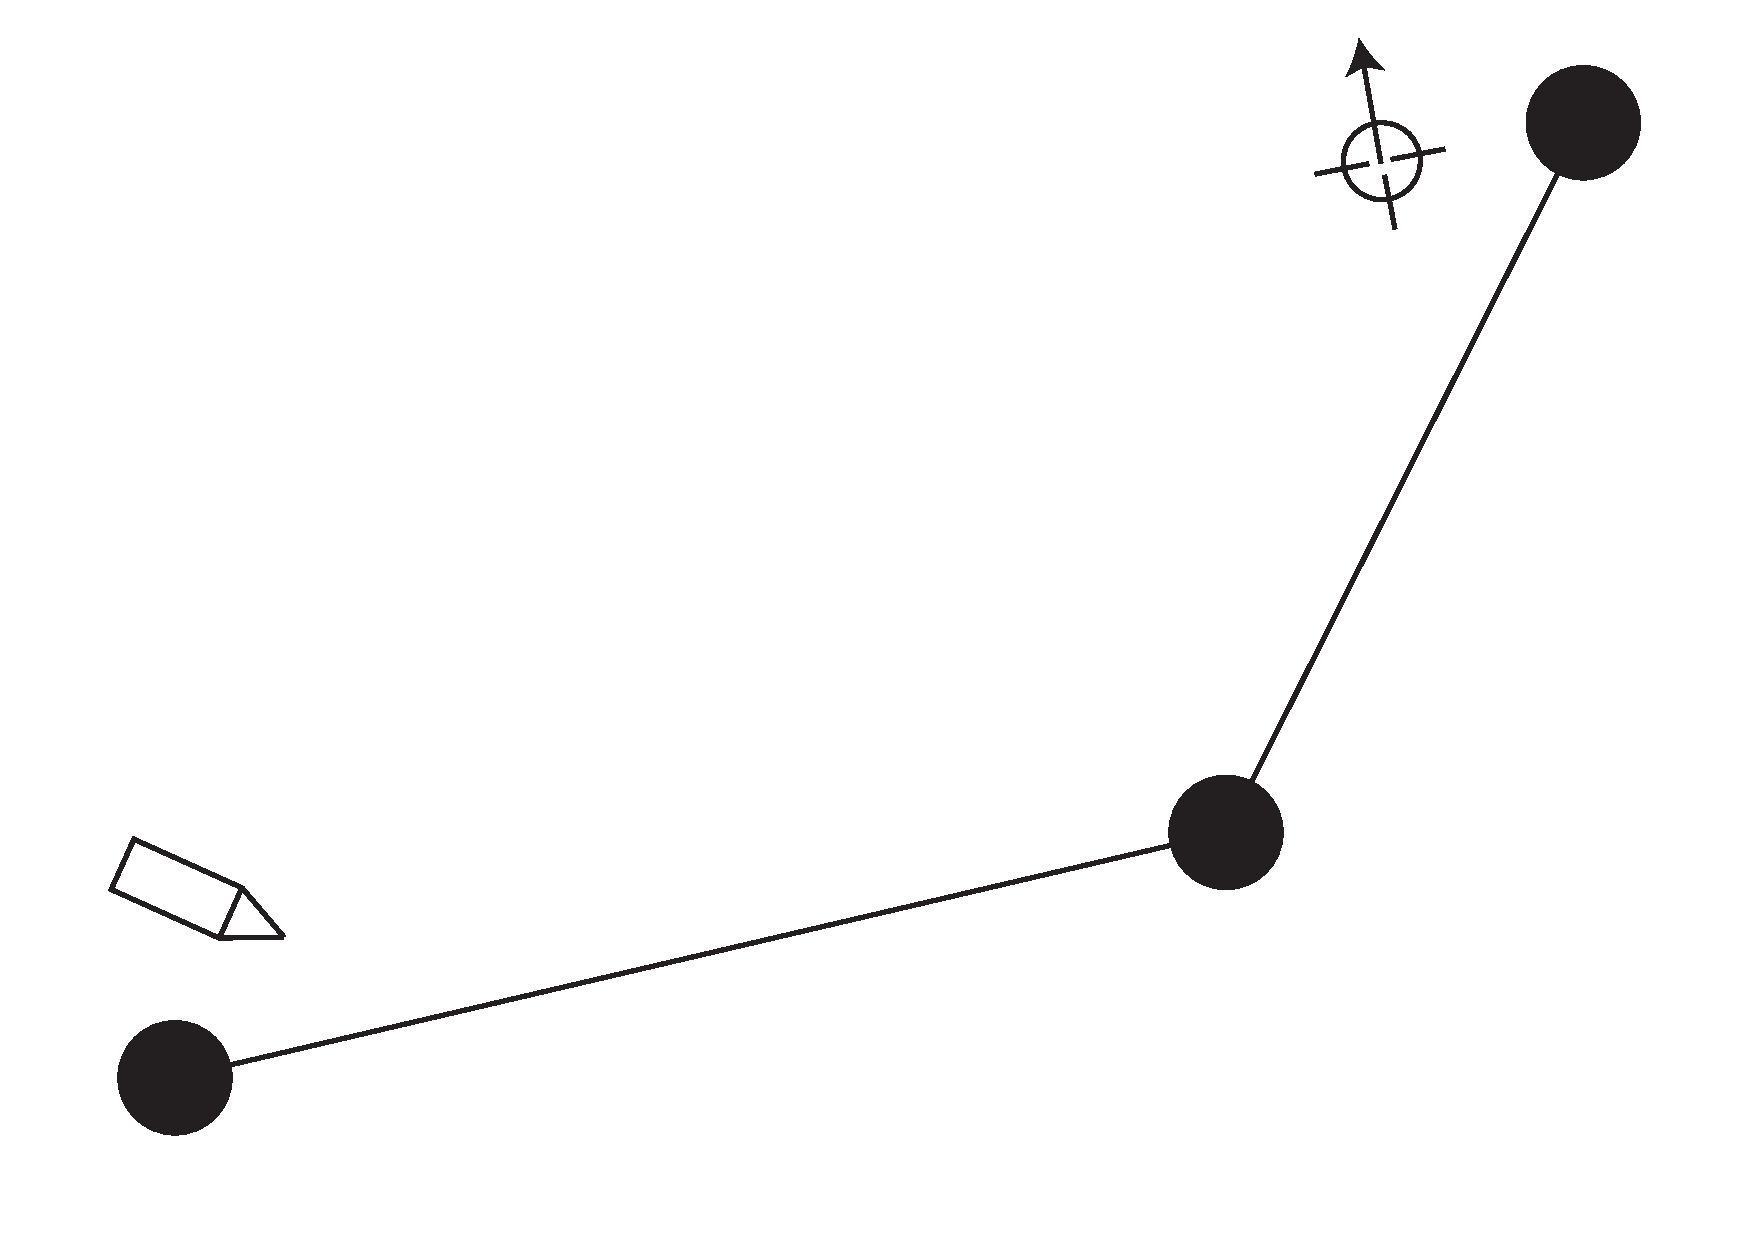
\includegraphics[width=20em]{res/pathfinding/spacelanes}
	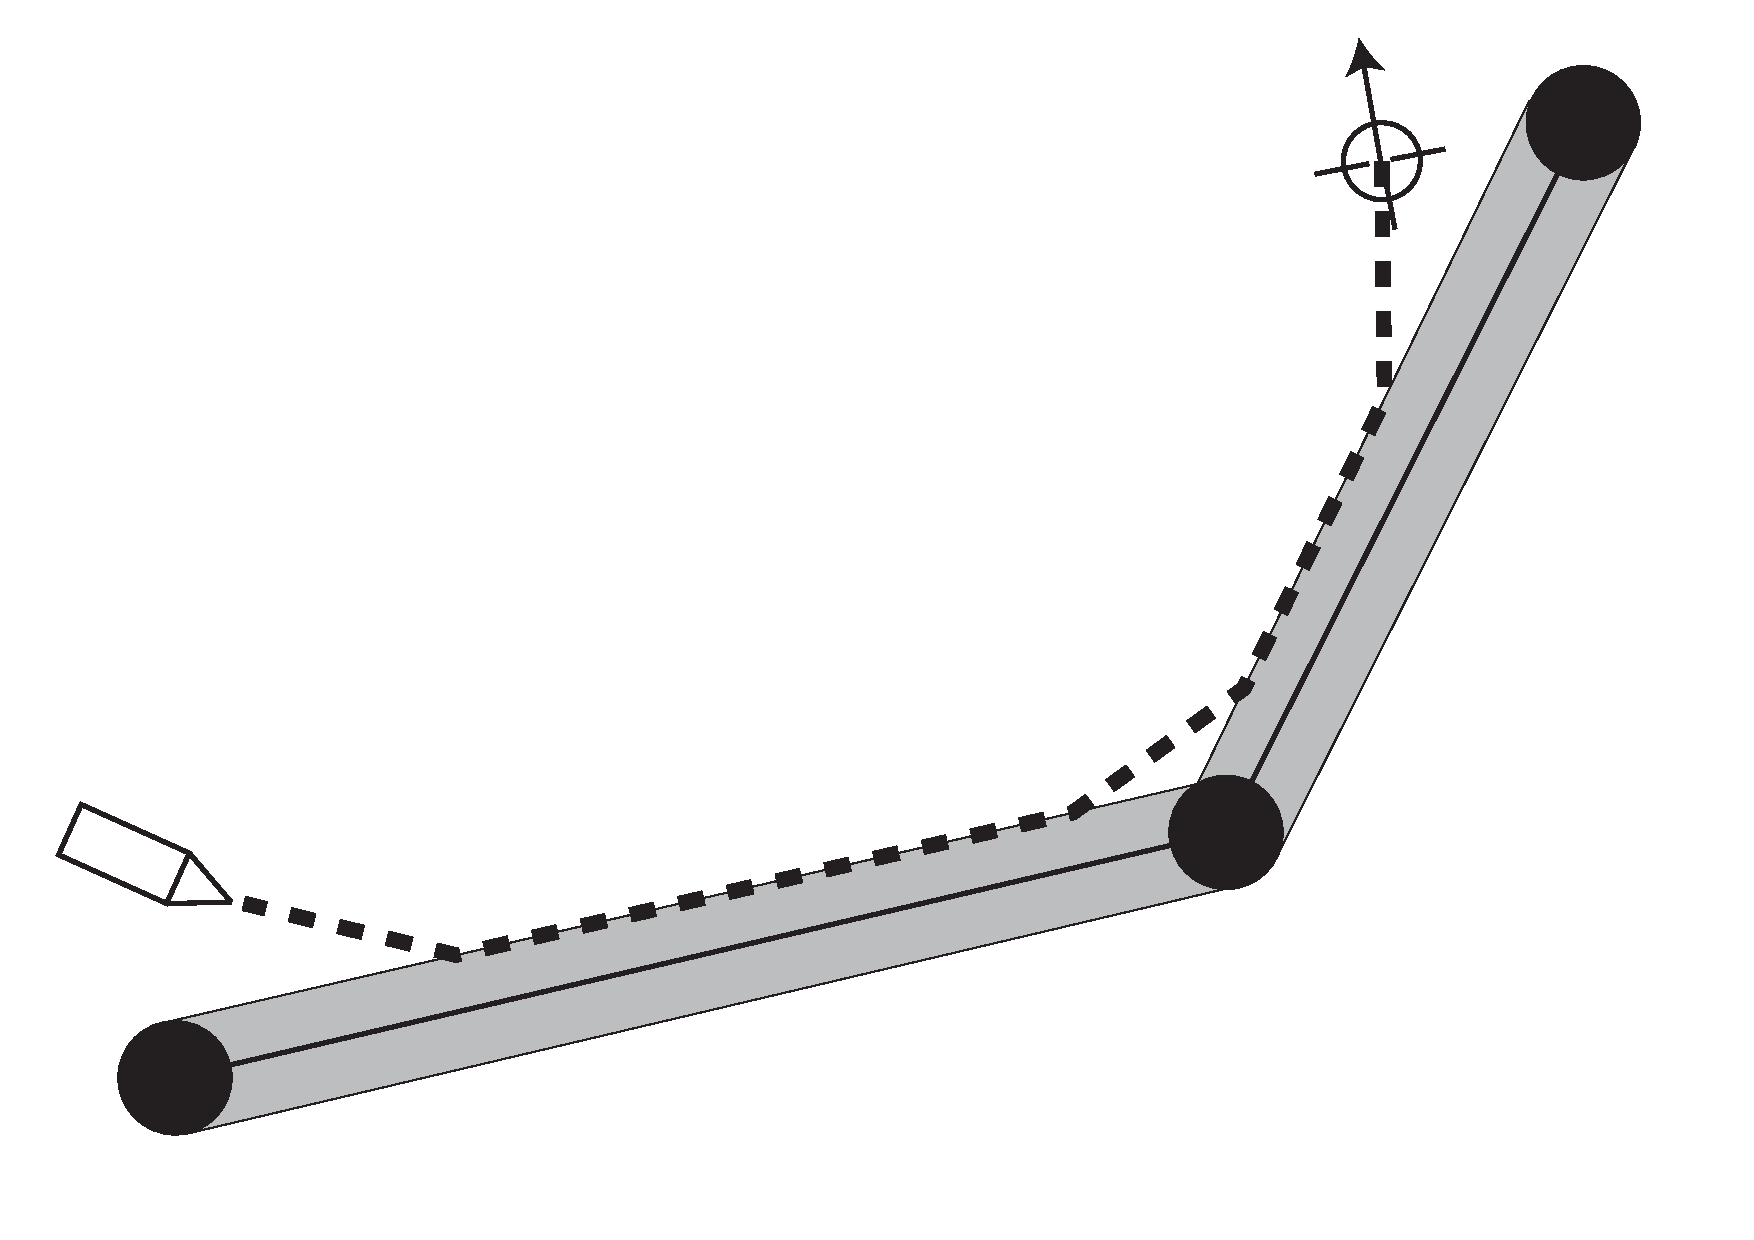
\includegraphics[width=20em]{res/pathfinding/spacelanes_ray}
	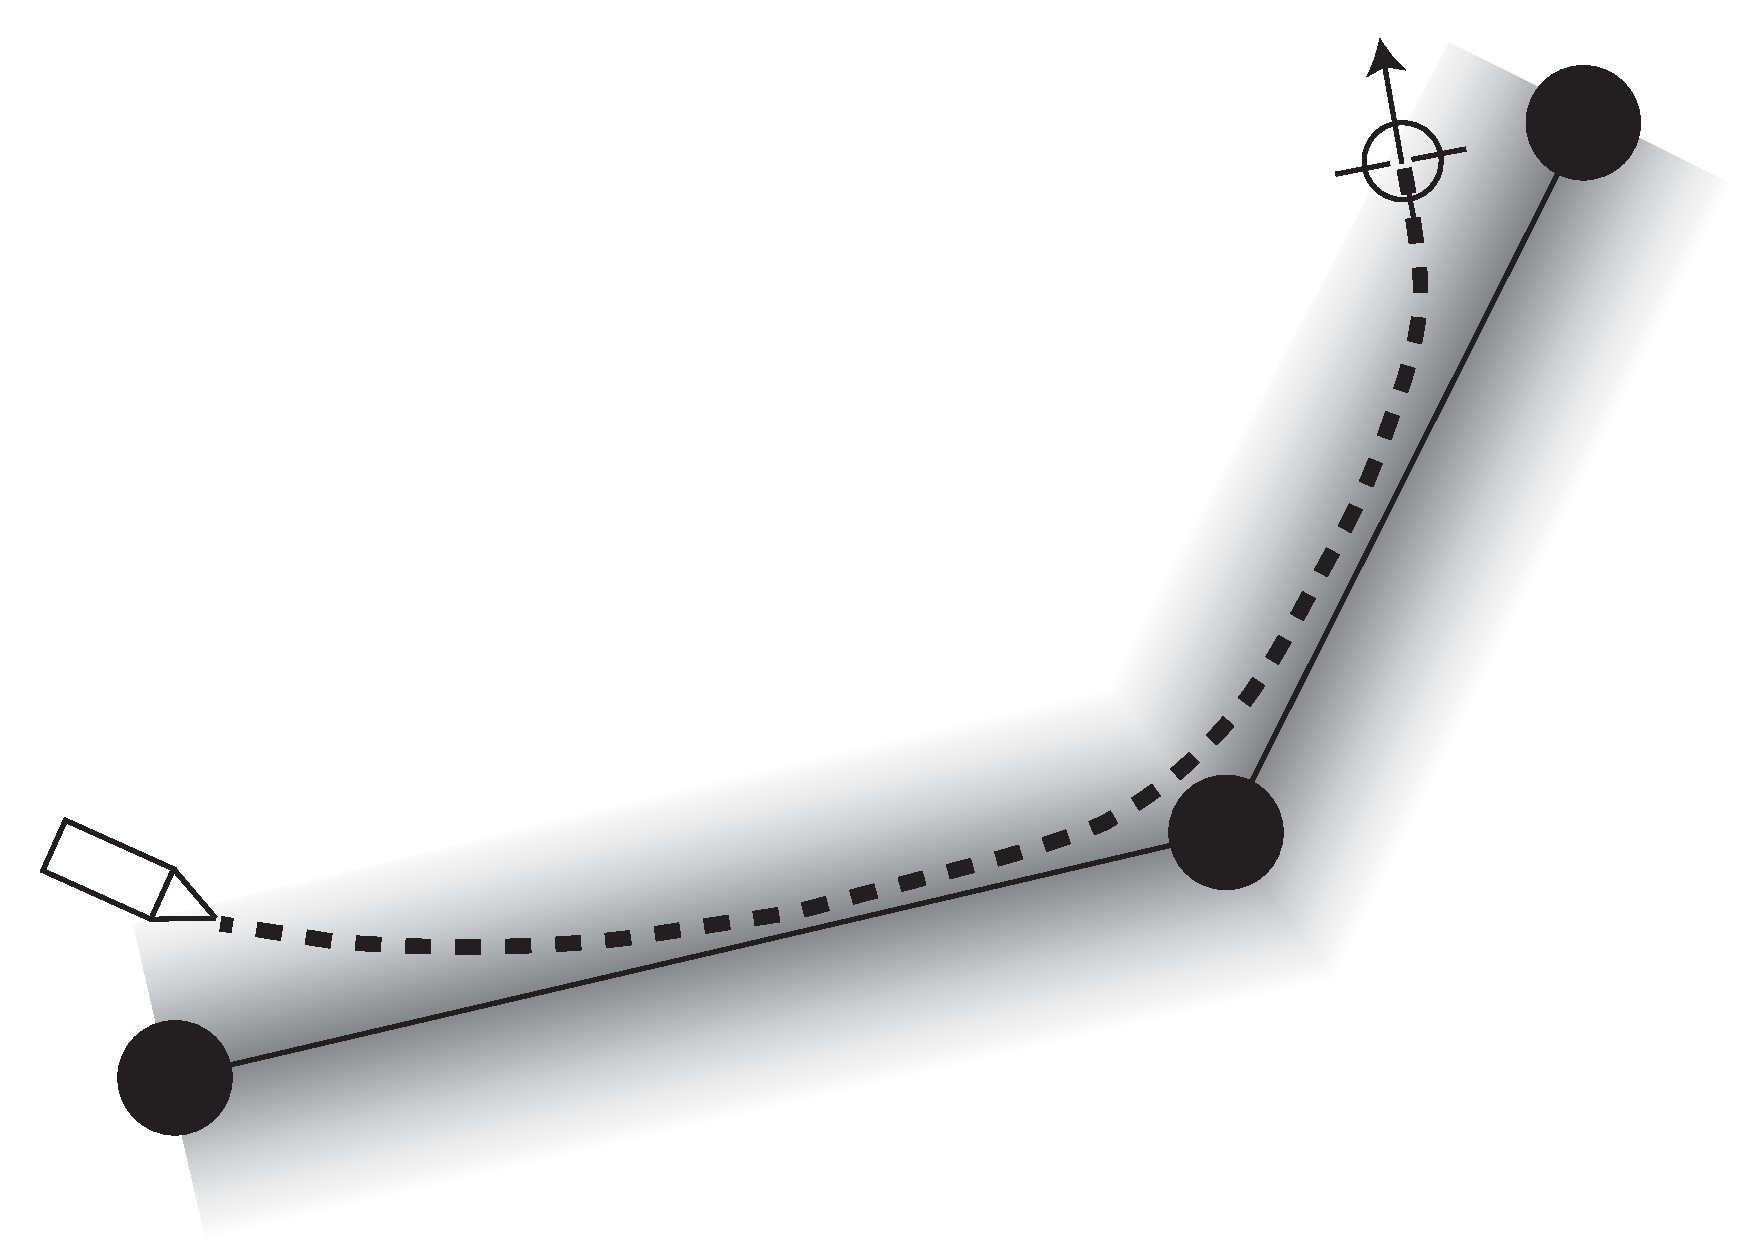
\includegraphics[width=20em]{res/pathfinding/spacelanes_field}
	\caption[Illustrations of different models for a path between current location and target utilising a space lane.]{Illustrations of different models for a path between current location and target utilising a space lane.}
	\label{fig:spacelanes}
\end{marginfigure}

Intimately related to these questions is the precise nature of the spacelane mechanics. Many different models were discussed for this during design meetings. Initial ideas on the physical mechanism of the spacelane was that they conferred an additional optional acceleration: i.e. that if a ship is proximate to a lane it could opt to undergo greater acceleration than a ship far from a lane. But as mentioned, accurately modelling acceleration in space is somewhat contrary to the gameplay aspirations of the design. 

A simpler mechanics for ships that was considered to be more suitable, is for them to have a top speed that they could reach relatively quickly; but for them to still have large turning circles. This makes their motion more similar to naval ships engaged in warfare. The interpretation of the spacelane in this model cannot be simply a gain in acceleration as this confers little benefit. Instead it is clear that the spacelane must confer an addition to top speed. A possible physical interpretation of these behaviours is that the ships are moving in some kind of ether with friction, and so will reach a terminal velocity. The spacelane is then an area with an  artificially induced lower density of ether.

Another fundamental question about the nature of the spacelane is whether its effects are immediately felt at full strength at a certain distance from it, or whether they fall off related to distance. the former is most definitely simpler, but the latter feels more natural as a mechanism. Figure~\ref{fig:spacelanes} shows the difference in the shortest paths that these approaches may generate, discounting the additional issue of ship turning.

\subsection{Algorithms for Pathfinding}
% physics hard
% bezier (not trivial)
% flow fields

\subsection{Applying A* to Sector}
% what is the problem
% why this is no trivial problem
% Why A*
Pathfinding for a game has 2 components: navigating a graph which represents the game, and the algorithm that traverses the graph to find the shortest route to a destination.
A* was chosen because it can guarantee an optimal solution, and it typically very fast if it has a good heuristic. 
Since the line of sight heuristic is applicative in this game A* will find most paths without expanding many nodes.
A* is designed to navigate discrete graphs, however In this game the sector is not a discrete graph.
The planets and space lanes on the sector can be considered a discrete graph however planets are not the only locations ships can exist at, they can move anywhere in the sector, the spaces lanes just provide a speed boost.

% conversion from sector to sector graph
A solution to this problem was to generate a discrete graph from the sector graph that could then be used by A* algorithm to find a path to destination. 
In a game such as Moon Survival on page {sec:rd:moonSurvival} the the world is already a discrete graph in the form of a 2-dimensional grid of squares, hence this can be traversed by the A* algorithm in place without having to generate a separate navigation graph.

Making a discrete navigation graph before A* could require considerable memory and CPU resources depending on the sector size.
An alternative to this solution would be to modify A* to traverse continuous graphs however designing a new algorithm to do this could cost considerable man hours to develop and will have no guarantees of finding a solution, let alone finding the optimal solution hence this alternative was dropped.

\begin{marginfigure}
	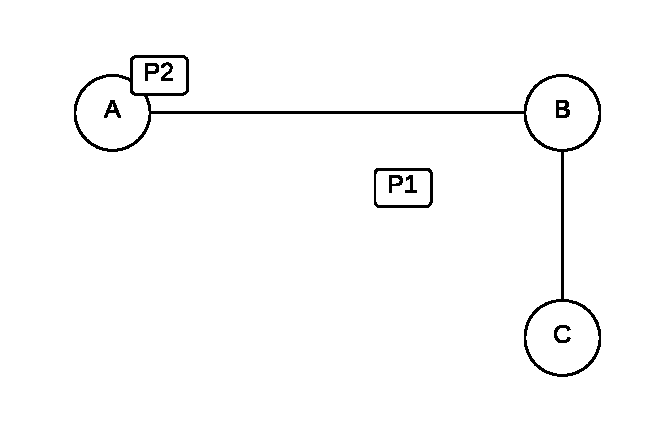
\includegraphics{res/pathfinding/PathFindingSector.pdf}
	\caption[Simple example of sector]{Simple example of sector with 3 planets: A, B, and C. Two points of interest are defined: P1 in the middle of the sector and P2 which is at planet A}
	\label{fig:pathfinding:simplesector}
\end{marginfigure}

%  - example 1
To work out how to generate a navigation graph from a sector, we needed to know the ideal path the ship would take under various circumstances before being able to implement it.
In Figure \ref{fig:pathfinding:simplesector} is an example of a sector with 3 planets.
If a ship is at P2 and wants to go to planet C, its seems rather obvious: take space lane to B then space lane to C. A space lane is faster to navigate than open space.

%  - example 2
Now consider a ship is at P1 and wants to go to planet C.
It has 3 obvious options:
\begin{itemize}
\item 
\begin{marginfigure}
	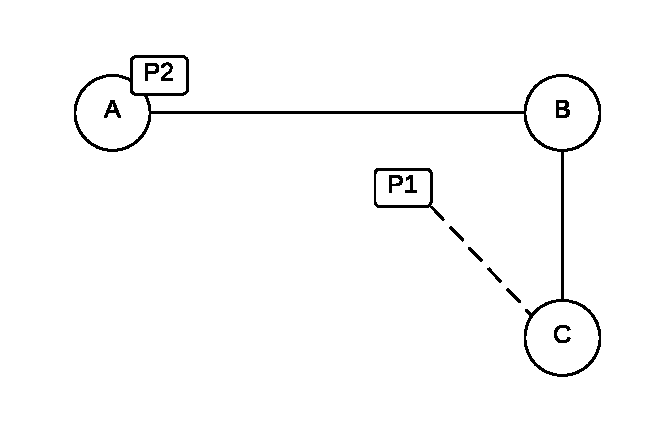
\includegraphics{res/pathfinding/PathFindingSectorOption1.pdf}
    \caption{sector navigation - option 1: path directory to planet C}
	\label{fig:pathfinding:simpleSectorOption1}
\end{marginfigure}
go directory to C across open space (Figure \ref{fig:pathfinding:simpleSectorOption1})

\item 
\begin{marginfigure}
	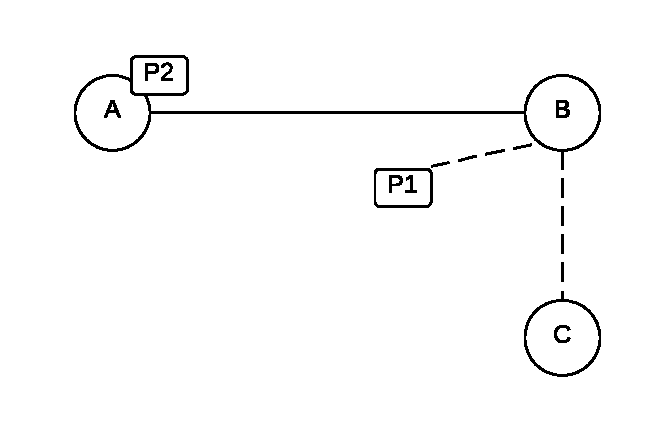
\includegraphics{res/pathfinding/PathFindingSectorOption2.pdf}
    \caption{sector navigation - option 2: path to B then to C}
	\label{fig:pathfinding:simpleSectorOption2}
\end{marginfigure}
goto Planet B which is close, then use its space lane to Planet C (Figure \ref{fig:pathfinding:simpleSectorOption2})

\item 
\begin{marginfigure}
	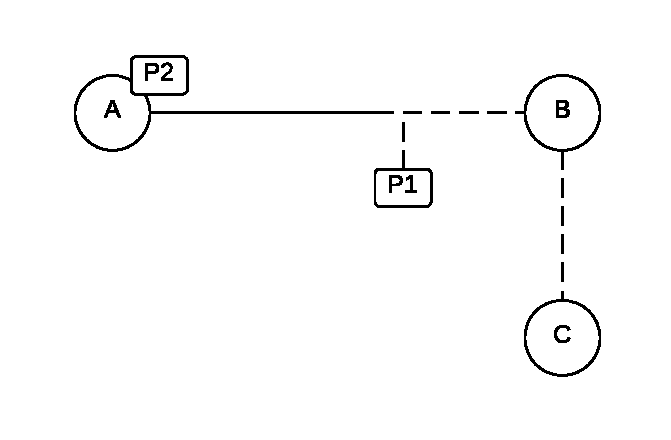
\includegraphics{res/pathfinding/PathFindingSectorOption3.pdf}
    \caption{sector navigation - option 3: path to space lane then to B then to C}
	\label{fig:pathfinding:simpleSectorOption3}
\end{marginfigure}
goto space lane between planet A and B and use it to got to B then use space lane to get to C (Figure \ref{fig:pathfinding:simpleSectorOption3}).

\end{itemize}

Traveling across open will always be considerable slow to space lanes so option 1 seems like a suboptimal choice, however did bring to light the question: How fast are space lanes?
The speed at which ships travel on space lanes needed to be defined in order to know which route is faster.

Every ship class could have 2 properties, one defining its speed in open space and one defining its speed on space lanes.
This method would allow the more specialisation amongst ships, allowing the concept of hit and run over space lanes. 
It seemed logical that a slow ship on open space should be slow on a space lane relative to a fast ship on open space, hence it seemed redundant to have 2 speed properties on a ship class.
The Method chosen was instead to define a sector property called multiplier which specifies how much faster ships are on space lanes relative to open space.
For example if the multiplayer was 3, then a ship with a speed of 10 in open space would have a speed of 30 on a space lane (3x10).
This multiplayer would be applied to all ships hence it would work on the ship's base speed defined on its ship class.
This method was simple and solved the problem.

back to the example of considering a ship at P1 which wants to go to planet C.
If we now assume a very large value for space lane multiplier, then it will greatly simplify these examples, then all space lanes will take approximately 0 seconds to use irrelevant to length, hence they are always faster over open space.
Under these conditions option 1 is slower then options 2 and 3.
Since P1 is closer to the space lane between A and B it would travel across less open space then traveling to B across open space, hence option 3 is faster then option 2.

\begin{marginfigure}
	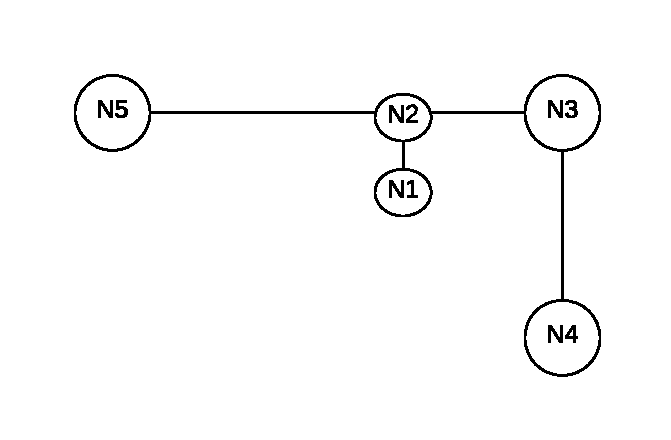
\includegraphics{res/pathfinding/PathFindingSectorOption3NavigationGraph.pdf}
    \caption[sector navigation - option 3 navigation graph]{sector navigation - option 3 navigation graph: each circle is node on navigation graph}
	\label{fig:pathfinding:simpleSectorOption3NavigationGraph}
\end{marginfigure}

To be able to generate a navigation graph that will allow option 3 to be a solution, the navigation graph in Figure \ref{fig:pathfinding:simpleSectorOption3NavigationGraph} would need to be generated.
In the graph their are only nodes. 
Nodes, N3, N4, and N5 were from the planets in Figure \ref{fig:pathfinding:simpleSectorOption3}.
Node N1 is the ship's starting point.
This needs to be added so the navigation graph is a connected graph.
If the destination wasn't a planet then a node would need to be added for this as well, but since the destination is a planet, no new node needs adding.

Node N2 doesn't correspond to any planet, start point or destination point, it corresponds to where the ship needs to enter the space lane.
It is a node that has no corresponding point on the original sector, it is a virtual node added to allow an optimal path to the solution.

The optimal solution is now: $N1 \to N2 \to N3 \to N4$.

For A* to make the same conclusion, costs needed to be associated with each edge on the navigation graph in Figure \ref{fig:pathfinding:simpleSectorOption3NavigationGraph}.
Since we want to minimise the time to destination, it makes sense to use time to traverse an edge.
To calculate the time to traverse an edge the following equation is used:
$$ time = \frac{distance}{speed} $$
The distance can easily be calculated using Pythagorean theorem, and the speed is simply the ship classes speed.
This works for open space edges but what about space lanes? obviously this will be much faster.
To make the formula work for both open space and space lanes the multiplayer needed to be factored in, giving the following formula:
$$ \frac{distance}{speed \times multiplier} $$
In open space the $multiplier$ is 1.0, and on space lanes it is whatever the sector defines it as.

% navigation of sector graph


% problems this method causes (not optimal solution but close)
% many nodes performance issues



